\section{Physical view}
In de physical view wordt er gekeken naar hoe het systeem gedeployed moet worden en waar.
Om dit in beeld te brengen is er gebruikgemaakt van een deployment diagram.
Het systeem wordt gedeployed met behulp van Docker containers.
Docker is een middel waarmee je software kan laten draaien op elke machine \Parencite{Docker}
Een representatie van de mogelijke deployement is te zien in figuur \ref{fig:DeploymentDiagram}.

\whitespace
\begin{graphic}
    \captionsetup{type=figure}
    \caption{Deployment diagram van het afstudeer product}
    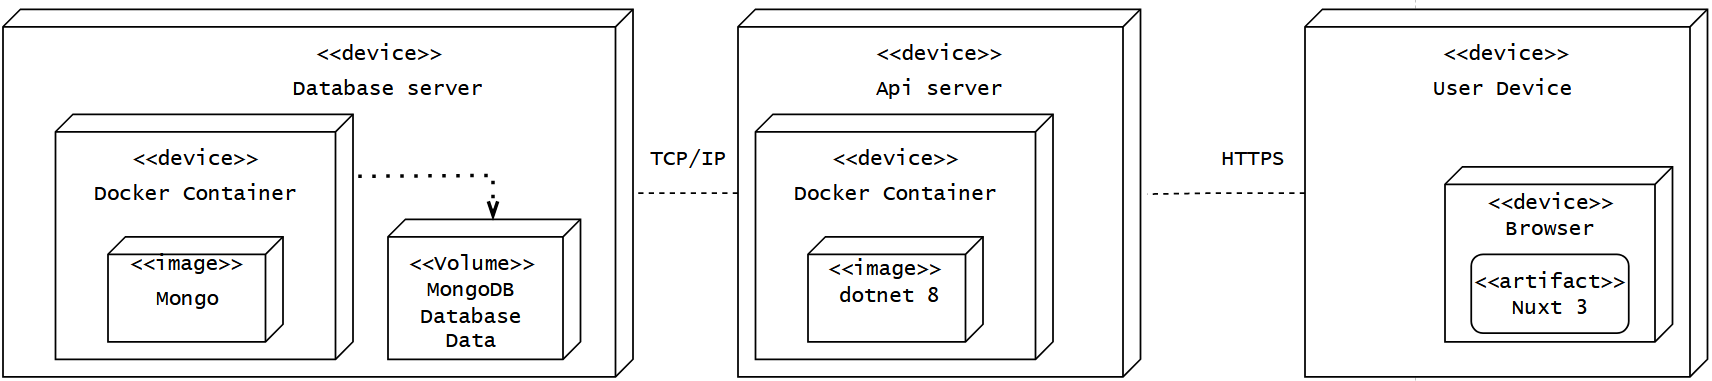
\includegraphics[scale=0.3]{DeploymentDiagram.png}
    \label{fig:DeploymentDiagram}
\end{graphic}
